\documentclass[tikz,border=2pt]{standalone}

\usepackage{amsmath} % for \text
\usepackage{xfrac} % for \myfrac
\usepackage{bm} % for \bm
\usetikzlibrary{calc}
\usetikzlibrary{positioning}
\usetikzlibrary{decorations.pathreplacing,decorations.markings}
\usetikzlibrary{patterns} % 加载 patterns 库
\usepackage{comment}


\colorlet{myred}{red!80!black}
\colorlet{myblue}{blue!80!black}
\colorlet{mygreen}{green!60!black}
\colorlet{myorange}{orange!70!red!60!black}
\colorlet{mydarkred}{red!30!black}
\colorlet{mydarkblue}{blue!40!black}
\colorlet{mydarkgreen}{green!30!black}
\colorlet{myred2}{red!50!white}

\colorlet{mylightblue}{blue!60!cyan!80!black!15}
\colorlet{mypurple}{blue!50!red!70}
\colorlet{gaugecol}{red!90!black!70} % Wiki red
\colorlet{leptoncol}{green!80!black!70} % Wiki green
\colorlet{quarkcol}{blue!85!cyan!95!black!55} % Wiki purple
\colorlet{quarkred}{red!98!black!55} % quark red
\colorlet{quarkblue}{blue!85!cyan!98!black!55} % quark blue
\colorlet{quarkgreen}{green!95!black!55} % quark green
\colorlet{gluoncyan}{cyan!100!black!55} % gluon cyan
\colorlet{gluongreen}{green!75!blue!95!black!70} % gluon green
\colorlet{gluonyellow}{yellow!98!black!55} % gluon yellow
\colorlet{gluonorange}{orange!100!black!65} % gluon orange
\colorlet{gluonmagenta}{magenta!100!black!70} % gluon magenta
\colorlet{scalarcol}{yellow!70!orange!98!black}
\colorlet{tensorcol}{blue!50!red!70} % Wiki light blue
\colorlet{groupcol}{orange!15}

\tikzset{
    mynode/.style={
        circle,        % 形状为圆形
        fill=black,    % 填充颜色为黑色
        inner sep=0.4, % 点的大小
        draw           % 添加边框
    }
}


\begin{document}

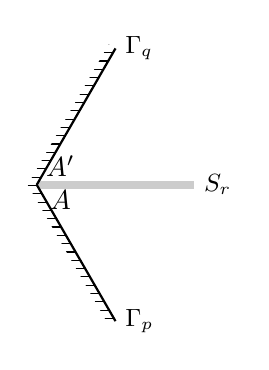
\begin{tikzpicture}[x=2cm, y=2cm]

\def\th{60}

\def\De{0.05}

% 定义点
\coordinate (P1) at (0,0);

\pgfmathsetmacro{\x}{1}
\pgfmathsetmacro{\y}{0}
\coordinate (P2) at (\x,\y);

\pgfmathsetmacro{\x}{cos(\th)}
\pgfmathsetmacro{\y}{-sin(\th)}
\coordinate (P3) at (\x,\y);

\pgfmathsetmacro{\x}{cos(\th)}
\pgfmathsetmacro{\y}{sin(\th)}
\coordinate (P4) at (\x,\y);

\pgfmathsetmacro{\x}{cos(\th)+\De*cos(-\th-90)}
\pgfmathsetmacro{\y}{sin(-\th)+\De*sin(-\th-90)}
\coordinate (P5) at (\x,\y);

\pgfmathsetmacro{\x}{cos(\th)+\De*cos(\th+90)}
\pgfmathsetmacro{\y}{sin(\th)+\De*sin(\th+90)}
\coordinate (P6) at (\x,\y);

\pgfmathsetmacro{\x}{-\De/sin(\th)}
\pgfmathsetmacro{\y}{0}
\coordinate (P7) at (\x,\y);

\pgfmathsetmacro{\x}{1}
\pgfmathsetmacro{\y}{-0.15}
\coordinate (P8) at (\x,\y);

\pgfmathsetmacro{\x}{1}
\pgfmathsetmacro{\y}{0.15}
\coordinate (P9) at (\x,\y);

\begin{scope}
\clip  (P1) -- (P3) -- (P8) -- (P9) -- (P4) -- cycle;
\draw[gray!40, line width=3.0] (P1) -- (P2);
\end{scope}

\fill[pattern=horizontal lines]
    (P1) -- (P4) -- (P6) -- (P7) -- (P5) -- (P3) -- cycle ;

\draw[thick] (P1) -- (P3);
\draw[thick] (P1) -- (P4);

\node[right] at (P3) {\small $\Gamma_p$};
\node[right] at (P4) {\small $\Gamma_q$};
\node[right] at (P2) {\small $S_r$};

\node[shift={(0.15, 0.12)}] at (P1) {$A^\prime$};
\node[shift={(0.15, -0.1)}] at (P1) {$A$};    
\fill (0, 0) circle[radius=0.0125cm];
 
\end{tikzpicture}


\end{document}